\textbf{\LARGE osn 17. Понятие архитектуры ЭВМ. Принципы фон Неймана. Компоненты компьютера: процессор, оперативная память, внешние устройства. Аппарат прерываний.}


\textbf{Компьютер} --- исполнитель алгоритма на языке машины.

\textbf{Архитектура ЭВМ} --- совокупность узлов машины и взаимосвязей между ними, рассматриваемая на определённом уровне рассмотрения этой архитектуры.

\textbf{Принципы фон Неймана:}
\begin{enumerate}
    \item Принцип двоичного кодирования информации: вся информация, которая поступает и обрабатывается в компьютере, кодируется в двоичной системе счисления.
    \item Принцип программного управления. Программа состоит из команд, в которых закодированы операция и операнды, над которыми должна выполниться данная операция. Выполнение компьютером программы — это автоматическое выполнение определенной последовательности команд, составляющих программу. В компьютере устройство, обеспечивающее выполнение команд, — Последовательность выполняемых процессором команд последовательностью команд и данных, составляющих программу. То есть, по сути, второй принцип – это принцип последовательной обработки.
    \item Принцип хранимой программы. Для хранения команд и данных программы используется единое устройство памяти, которое представляется в виде вектора слов. Все слова имеют последовательную адресацию. Команды и данные представляются единым образом. Интерпретация информации памяти и, соответственно, ее идентификация как команды или как данных происходит неявно при выполнении очередной команды. К примеру, содержимое слова, адрес которого используется в команде перехода в качестве операнда, интерпретируется как команда. Если то же слово используется в качестве операнда команды сложения, то его содержимое интерпретируется как данные. То есть одна и та же область памяти в зависимости от команд в одном случае будет интерпретироваться как команда, в другом случае – как данные. Этот принцип фон Неймана замечателен тем, что он определяет возможность программной генерации команд с последующим их выполнением, то есть возможность компиляции программы, когда одна программа порождает другую программу, которая будет выполняться.
\end{enumerate}

\textbf{Процессор} состоит из \textit{устройства управления (УУ)} и \textit{арифметико-логического устройства (АЛУ)}. АЛУ выполняет различные операции над данными, хранящимися на регистрах АЛУ. УУ выполняет команды языка машины, посылая управляющие сигналы к остальным устройствам.

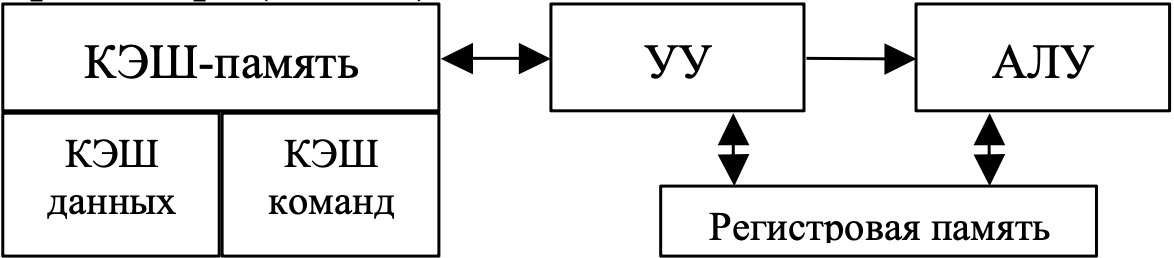
\includegraphics[width=\columnwidth]{pics/CPU.png}

\textbf{Основная (оперативная) память} хранит команды программы и обрабатываемые данные. ОЗУ состоит из ячеек, ячейка памяти - устройство, в котором размещается информация. Ячейка состоит из двух полей \textit{тег} и \textit{машинное слово}. Машинное слово - поле программно изменяемой информации. Здесь могут располагаться машинные команды или данные, с которыми будет оперировать программа. Имеет фиксированный для данной ЭВМ размер. Размер машинного слова - количество двоичных разрядов, размещаемых в машинном слове. Поле машинной информации (тег) - поле ячейки памяти, в котором схемами контроля процессами и ОЗУ автоматически размещается информация, необходимая для осуществления контроля за целостностью и корректностью использования данных. Использование тега:
\begin{itemize}
    \item Контроль за целостностью данных - одноразрядный тег, который использовался для контроля точности.
    \item Контроль доступа к командам/данным. (вся информация раскрашивается в 2 цвета - команды и данные)
    \item Контроль доступа к машинным типам данных. (в теге записывается код типа данных)
\end{itemize}

Ячейки памяти, расположенные не в основной памяти ЭВМ, а в других устройствах, называются регистрами. В процессе работы команды поступают на регистры в УУ, а данные --- на регистры в АЛУ. АЛУ может обрабатывать данные только на своих регистрах, чтобы обработать данные, расположенные в основной памяти, их надо сначала считать на регистры в АЛУ.

\textbf{Внешние устройства} служат для обмена программами и данными между основной (оперативной) памятью и <<внешним миром>>.


\centerline{\textbf{Аппарат прерываний}}

\textbf{Аппарат прерываний} -- способность ЭВМ быстро и гибко реагировать на события, происходящие как внутри процессора и оперативной памяти, так и во внешних устройствах. Каждое такое событие порождает сигнал, приходящий на специальную электронную схему -- контроллер прерываний.

Прерывания делятся на:
\begin{itemize}
    \item[--] \textit{Внутренние (синхронные)}, источником которых являются выполняемые команды программы, их нельзя закрыть и не реагировать на них.
    \item[--] \textit{Внешние (асинхронные)}, которые вызываются событиями в периферийных устройствах. Эти прерывания можно временно закрыть, если в данный момент процессор занят другой срочной работой.
\end{itemize}
    
\textbf{Аппаратная реакция} на прерывание заключается в сохранении информации о считающейся в данное время программе (процесса) и переключение на выполнение другой программы (процедуры обработки прерывания, т.е. события, здесь включается режим блокировки прерываний). В некоторых архитектурах это называется переключением контекста. Этот механизм позволяет (при необходимости) продолжить (возобновить) выполнение прерванной программы с текущего места.

\textbf{Программная реакция} на прерывание производится процедурой-обработчиком прерывания и делится на два этапа. Сначала происходит минимальная программная реакция, она производится в режиме с закрытыми прерываниями от внешних устройств. Это опасный режим, так как процессор не обращает внимание на все события в периферийных устройствах. Затем происходит полная программная реакция уже в режиме с открытыми прерываниями.

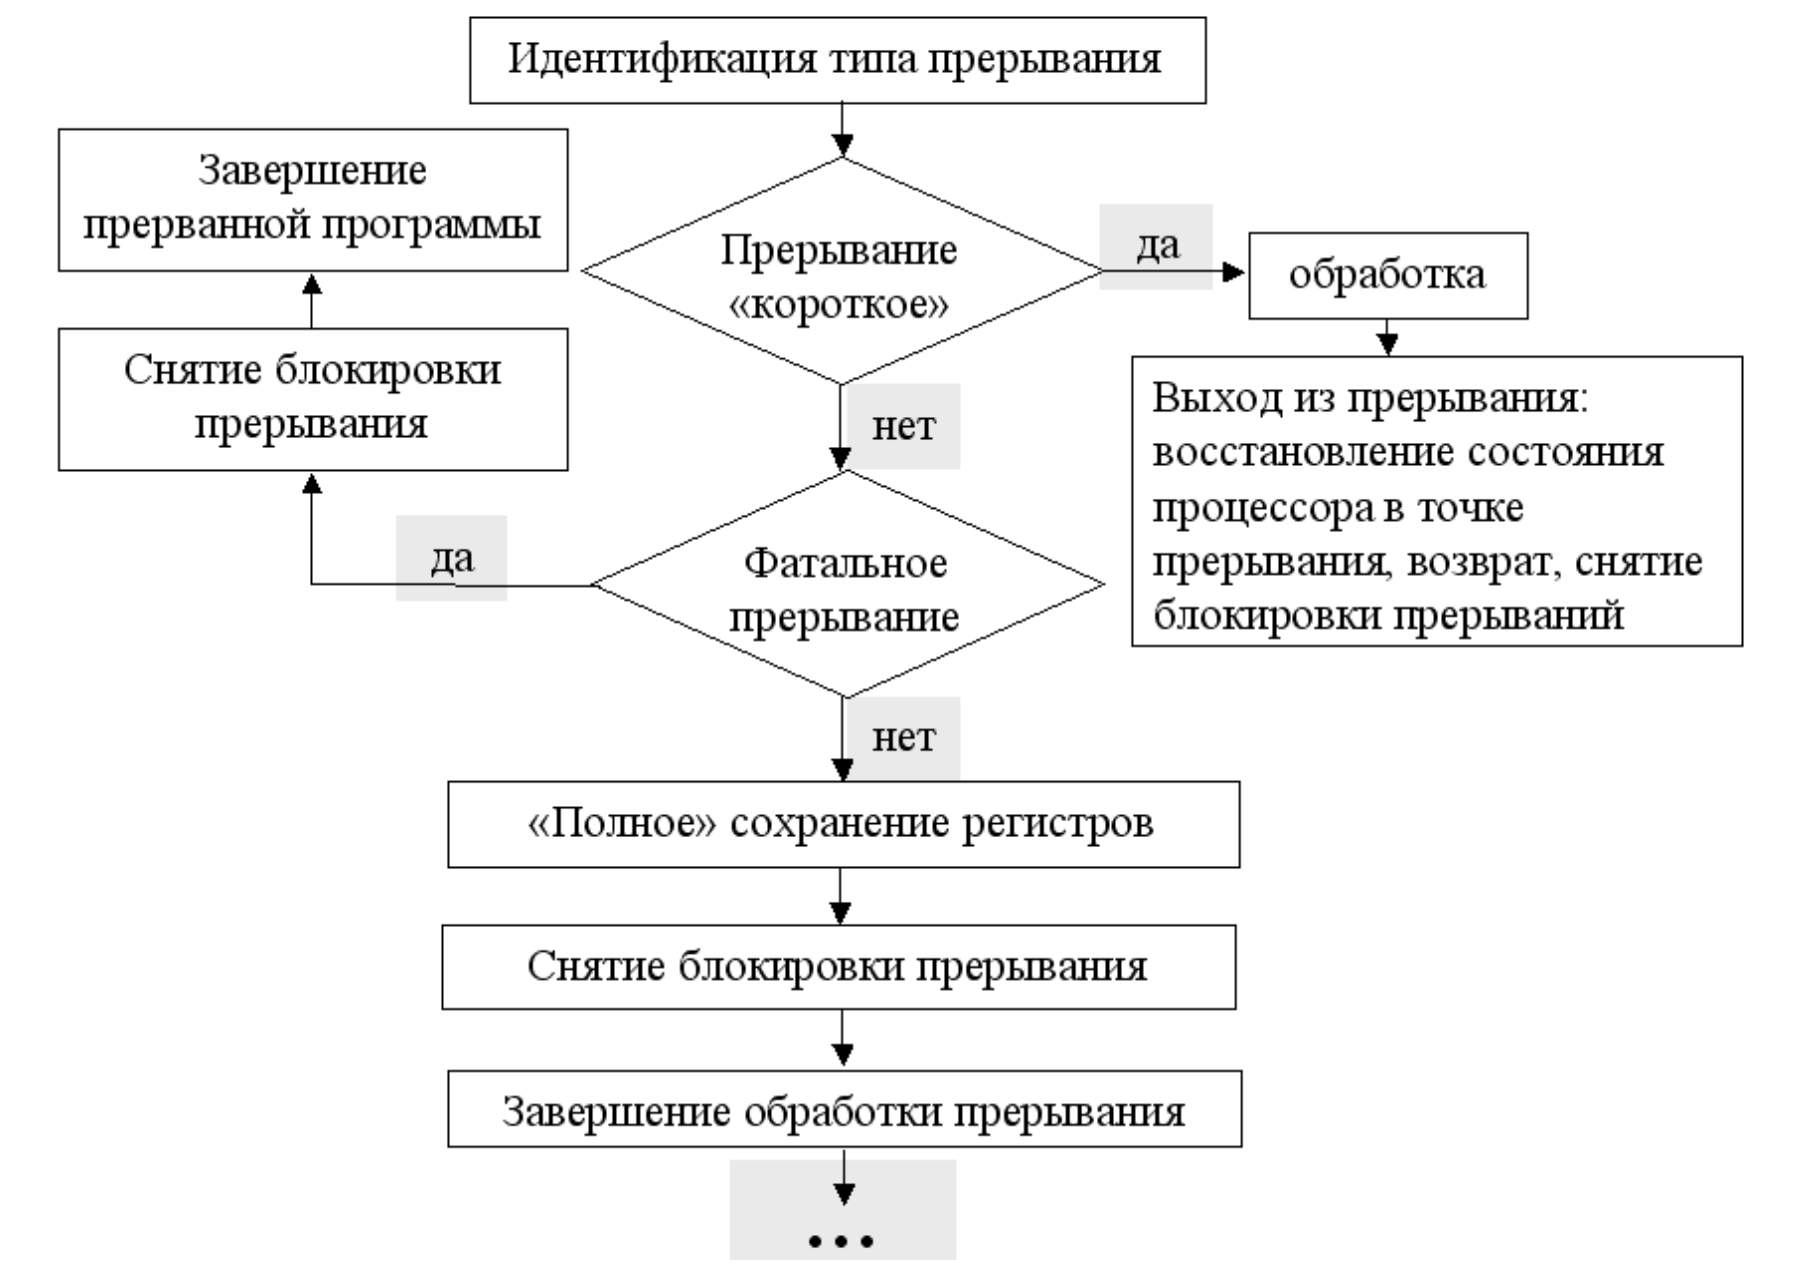
\includegraphics[scale=0.31]{pics/interruptions.png}

\textbf{Короткое прерывание} -- обработка не требует дополнительных ресурсов ЦП и времени.

\textbf{Фатальное прерывание} -- после него продолжить выполнение программы невозможно.


% % -------- source --------
% \bigbreak
% [\cite[page 69-96]{replace_me}]